\documentclass[a4paper, 12pt]{article}

%\usepackage{cmap}
\usepackage[T2A]{fontenc}
\usepackage[utf8]{inputenc}
\usepackage[english, russian]{babel}
\usepackage{graphicx}
\usepackage[top=1in, bottom=1in, left=3.2cm, right=2.6cm]{geometry}
\graphicspath{./}
\usepackage{biblatex}
\addbibresource{lib.bib}
\linespread{1.5}
\usepackage{ragged2e}
\justifying
\usepackage{listings}
\usepackage{color}


\begin{document}
	
\begin{titlepage}
	\fontsize{12pt}{12pt}\selectfont
	\begin{figure}[t!]
		\centering
		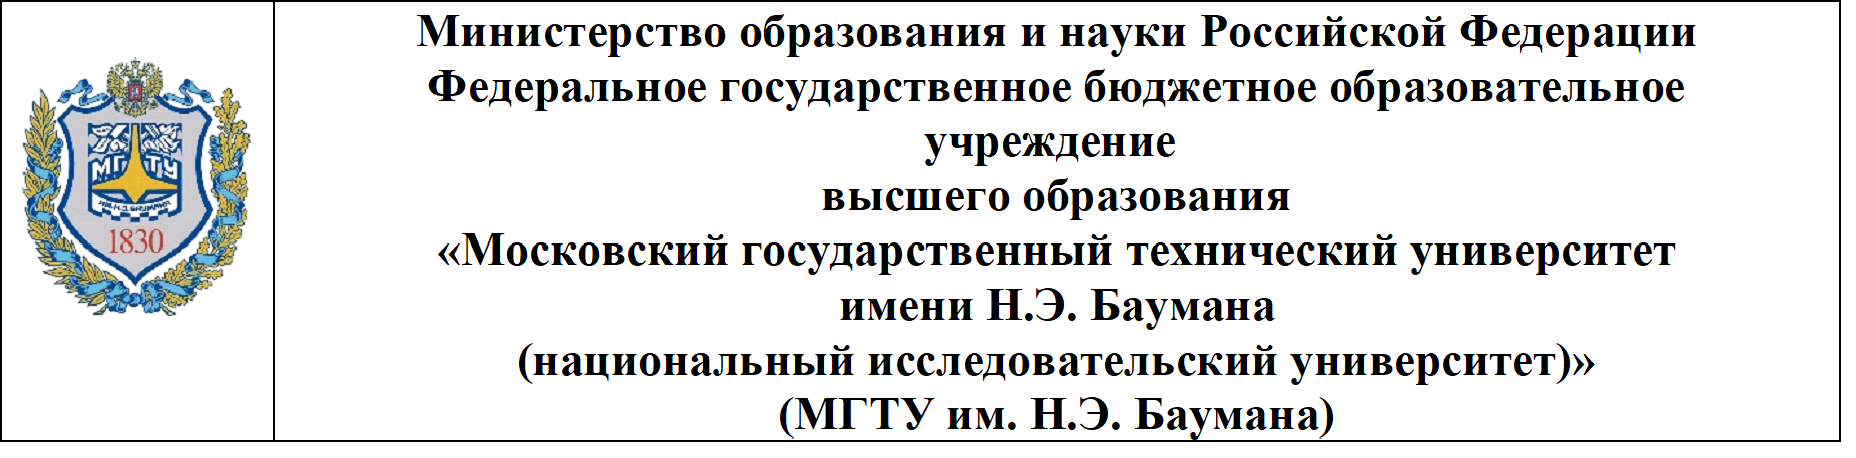
\includegraphics[scale=0.8]{bmstu}
	\end{figure}
	
	\noindent\rule{15cm}{3pt}
	\newline\newline
	\noindent 
	ФАКУЛЬТЕТ 
	\underline{«Информатика и системы управления»} \newline\newline
	
	\noindent КАФЕДРА \underline{«Программное обеспечение ЭВМ и информационные технологии»}\newline\newline\newline\newline\newline
	
	\centering {\Large Отчет по лабораторной работе № 10}
	\vspace{4mm}
	
	\centering {\Large По курсу: "Функциональное и логическое программирование"
		\vspace{8mm}	
		
		}
	\vspace{8mm}
	
	
	\begin{flushright}
		{\small	Студент:\\ Турсунов Жасурбек Рустамович \\ Группа: ИУ7-66Б
			\vspace{3mm}
			\\Преподователи: \\ Толпинская Наталья Борисовна \\ Строганов Юрий Владимирович}
	\end{flushright}
	
	\begin{center}
		\vfill
		Москва, \the\year
		~г.
	\end{center}
\end{titlepage}

\tableofcontents
\clearpage
\newpage

\textbf{Цель работы:} приобрести навыки организации сложных рекурсивных функций с использованием функционалов.
\\ \hspace*{5mm} \textbf{Задачи работы:} изучить способы применения функционалов и рекурсии при обработке одноуровневых и структурированных списков.


\section*{Введение}
\addcontentsline{toc}{section}{Введение}

\hspace*{5mm} Для организации многократных вычислений в Lisp могут быть использованы функционалы - функции, которые особым образом обрабатывают свои аргументы. Функционалы - это  функции более высокого порядка, так как они в качестве своего первого аргумента принимают функциональный объект - функцию, имеющую имя(глобально определенную функцию), или функцию, не имеющею имени(локально определенную функцию). При использовании рекурсии - необходимо обеспечить эффективность работы, путем использования хвостовой рекурсии. В рекурсивных функциях могут быть использованы дополнительные функции - не в аргументах вызова, а вне них. Рекурсивные вызовы могут быть организованы как в одной ветке, так и в нескольких ветках программы. Рекурсивные функции могут вызывать друг друга.  функционалы, являющиеся предикатами, функционалы, использующие предикаты в качестве функционального объекта
\clearpage
\newpage


\definecolor{codegreen}{rgb}{0,0.6,0}
\definecolor{codegray}{rgb}{0.5,0.5,0.5}
\definecolor{codepurple}{rgb}{0.58,0,0.82}
\definecolor{backcolour}{rgb}{0.95,0.95,0.92}

\lstdefinestyle{mystyle}{
	backgroundcolor=\color{backcolour},   
	commentstyle=\color{codegreen},
	keywordstyle=\color{magenta},
	numberstyle=\tiny\color{codegray},
	stringstyle=\color{codepurple},
	basicstyle=\ttfamily\footnotesize,
	breakatwhitespace=false,         
	breaklines=false,                 
	captionpos=b,                    
	keepspaces=true,                 
	numbers=left,                    
	numbersep=5pt,                  
	showspaces=false,                
	showstringspaces=false,
	showtabs=false,                  
	tabsize=4
}

\lstset{style=mystyle}

\section*{Задание 1}
\addcontentsline{toc}{section}{Задание 1}
Написать рекурсивную версию (с именем rec-add) вычисления суммы чисел заданного списка.
\subsubsection*{Хвостовая рекурсия:}
\begin{lstlisting}[caption=Функция-обертка для вычисления суммы чисел списка]
(defun rec-add (lst)
	(rec-add-helper lst 0)
)
\end{lstlisting}
\textbf{lst} - входной список.
\begin{lstlisting}[caption=Функция вычисления суммы чисел списка]
(defun rec-add-helper (lst sum)
	(cond	
		(
			(null lst) 
			sum
		)
		(
			(listp (car lst)) 
			(rec-add-helper (cdr lst) (rec-add-helper (car lst) sum)) )
		(
			(numberp (car lst)) 
			(rec-add-helper	(cdr lst) (+ sum (car lst)))
		)
		(
			(rec-add-helper (cdr lst) sum)
		)
	)
)
\end{lstlisting}
\textbf{lst} - входной список, \textbf{sum} - сумма чисел списка.

Условием выхода из рекурсии является достижение конца списка (первый аргумент - nil) - возвращается второй аргумент, в котором накапливается сумма чисел списка. Иначе, если голова первого аргумента список, то осуществляется рекурсивный вызов текущей функции для хвоста первого аргумента и рекурсивного вызова, который осуществляется для головы первого аргумента и второго аргумента. Если голова первого аргумента - число, то осуществляется рекурсивный вызов текущей функции для хвоста списка и суммы второго аргумента и головы первого аргумента. Если голова первого аргумента не число и не список, то осуществляется рекурсивный вызов текущей функции для хвоста первого аргумента и второго аргумента.
\subsubsection*{Примеры работы:}
\begin{lstlisting}
	> (rec-add '(1))
	1
	> (rec-add nil)
	0
	> (rec-add '(1 2 3))
	6
	> (rec-add '(1 2 (3 4) (5 (6))))
	21
	> (rec-add '(1 2 (a b (3)) nil (2 0)))
	8
\end{lstlisting}


\section*{Задание 2}
\addcontentsline{toc}{section}{Задание 2}
Написать рекурсивную версию с именем rec-nth функции nth.
\begin{lstlisting}[caption=Рекурсивная версия функции nth]
(defun rec_nth (lst n)
	(cond 
		( 
			(null lst) 
			nil
		)
		(
			(= n 0)
			(car lst)
		)
		(
			(rec_nth (cdr lst) (- n 1))
		)
	)
)
\end{lstlisting}
\textbf{lst} - входной список, \textbf{n} - индекс элемента, который нужно получить (начиная с 0).

Условиями выхода из рекурсии являются:
\begin{itemize}
	\item достижение конца списка(первый аргумент функции - nil) - возвращается nil;
	\item нахождение искомого элемента списка (второй аргумент функции равен 0) - возвращается этот элемент. 
\end{itemize} 
Иначе осуществляется рекурсивный вызов текущей функции для хвоста первого аргумента и второго аргумента, уменьшенного на 1.

\subsubsection*{Примеры работы:}
\begin{lstlisting}
	> (rec_nth nil 10)
	NIL
	> (rec_nth '(1) 0)
	1
	> (rec_nth '(1 (2 3) (4) 5 6) 1)
	(2 3)
	> (rec_nth '(1 2 3) 10)
	NIL
\end{lstlisting}

\section*{Задание 3}
\addcontentsline{toc}{section}{Задание 3}
Написать рекурсивную функцию alloddr, которая возвращает t, когда все элементы списка нечетные.

\subsubsection*{Хвостовая рекурсия:}
\begin{lstlisting}[caption=Функция-обертка проверки на нечетность всех элементов списка]
	(defun alloddr (lst)
	(alloddr-helper lst t)
	)
\end{lstlisting}
\textbf{lst} - входной список.
\begin{lstlisting}[caption=Функция проверки на нечетность всех элементов списка]
(defun alloddr-helper (lst isodd)
	(cond	
		(
			(or (null lst)(not isodd))
			isodd
		)
		(
			(listp (car lst))
			(alloddr-helper 
			(cdr lst) 
			(alloddr-helper (car lst) isodd))
		)
		(
			(and 
				(numberp (car lst))
				(oddp (car lst))
			)
			(alloddr-helper (cdr lst) isodd)
		)
	)
)
\end{lstlisting}
\textbf{lst} - входной список, \textbf{isodd} - логическая переменная для определения, содержаться ли в списке только нечетные числа, или нет.

По умолчанию считается, что список состоит только из нечетных чисел, поэтому начальное значение \textbf{isodd} - t.

Условием выхода из рекурсии является достижение конца списка(первый аргумент - nil) или нахождение элемента, являющего не нечетным(второй аргумент - nil) - возвращается второй аргумент. Если голова первого аргумента список, то осуществляется рекурсивный вызов текущей функции для хвоста первого аргумента и рекурсивного вызова, который осуществляется для головы первого аргумента и второго аргумента. Иначе, если голова первого аргумента - нечетное число, то осуществляется рекурсивный вызов текущей функции для хвоста списка и второго аргумента.

\subsubsection*{Примеры работы:}
\begin{lstlisting}
	> (alloddr nil)
	T
	> (alloddr '(1))
	T
	> (alloddr '(1 2))
	NIL
	> (alloddr '(1 3))
	T
	> (alloddr '(1 (3 (5) 7) 9))
	T
	> (alloddr '(1 (3 nil) 2))
	NIL
\end{lstlisting}


\section*{Задание 4}
\addcontentsline{toc}{section}{Задание 4}
Написать рекурсивную функцию, относящуюся к хвостовой рекурсии с одним тестом завершения, которая возвращает последний элемент списка-аргумента.
\begin{lstlisting}[caption=Функция получения последнего элемента списка]
(defun get_last (lst)
	(cond 
		(
			(null (cdr lst))
			(car lst)
		)
		(
			(get_last (cdr lst))
		)
	)
)
\end{lstlisting}
\textbf{lst} - входной список.

Условием выхода из рекурсии является достижение конца списка (хвост аргумента функции - nil) - возвращается голова аргумента. Иначе осуществляется рекурсивный вызов текущей функции для хвоста аргумента.

\subsubsection*{Примеры работы:}
\begin{lstlisting}
	> (get_last nil)
	NIL
	> (get_last '(1))
	1
	> (get_last '(1 2 3 4 5))
	5
	> (get_last '(1 2 (3 4) (5) 6 7))
	7
	> (get_last '(1 2 (3 4)))
	(3 4)
\end{lstlisting}



\section*{Задание 5}
\addcontentsline{toc}{section}{Задание 5}
Написать рекурсивную функцию, относящуюся к дополняемой рекурсии с одним тестом завершения, которая вычисляет сумму всех чисел от 0 до n-ого аргумента функции. 
\begin{lstlisting}[caption=Функция вычисления суммы элементов от 0 до n-го]
(defun sum_to_n (lst n)
	(cond
		(
			(or (= n 0)(null lst))
			0
		)
		(
			(+ 
				(car lst)
				(sum_to_n (cdr lst) (- n 1))
			)
		)	
	)
)	
\end{lstlisting}
\textbf{lst} - входной список, \textbf{n} - индекс элемента, до которого нужно производить сложение.

Условием выхода из рекурсии является достижение конца списка(первый аргумент функции - nil) или достижение нужного элемента(второй аргумент функции - 0) - возвращается 0. Иначе осуществляется рекурсивный вызов текущей функции для хвоста первого аргумента и второго аргумента, уменьшенного на 1, и возвращается сумма результата рекурсивного вызова и головы первого аргумента.
\subsubsection*{Примеры работы:}
\begin{lstlisting}
	> (sum_to_n nil 1)
	0
	> (sum_to_n '(1) 1)
	1
	> (sum_to_n '(1 2 3 4 5 6) 3)
	6
\end{lstlisting}

\section*{Задание 6}
\addcontentsline{toc}{section}{Задание 6}
Написать рекурсивную функцию, которая возвращает последнее нечетное число из числового списка, возможно создавая некоторые вспомогательные функции.

\begin{lstlisting}[caption=Функция-обертка для получения последнего нечетного числа]
(defun get_last_odd (lst)
	(get_odd lst nil)
)
\end{lstlisting}
\textbf{lst} - входной список.
\begin{lstlisting}[caption=Функция получения последнего нечетного числа]
(defun get_odd (lst num)
	(cond	
		(
			(null lst) 
			num
		)
		(
			(oddp (car lst))
			(get_odd (cdr lst) (car lst))
		)
		(
			(get_odd (cdr lst) num)
		)
	)
)
\end{lstlisting}
\textbf{lst} - входной список, \textbf{num} - последнее найденное нечетное число.

Условием выхода из рекурсии является достижение конца списка(первый аргумент - nil) - возвращается второй аргумент. Иначе осуществляется проверка на нечетность головы первого аргумента, если он нечетный, то осуществляется рекурсивный вызов текущей функции для хвоста первого аргумента и головы первого аргумента, если четный - осуществляется рекурсивный вызов для хвоста первого аргумента и второго аргумента.
\subsubsection*{Примеры работы:}
\begin{lstlisting}
	> (get_last_odd nil)
	NIL
	> (get_last_odd '(1))
	1
	> (get_last_odd '(1 2 3))
	3
	> (get_last_odd '(1 2 3 4 5 6))
	5
\end{lstlisting}


\section*{Задание 7}
\addcontentsline{toc}{section}{Задание 7}
Используя cons-дополняемую рекурсию с одним тестом завершения, написать функцию которая получает как аргумент список чисел, а возвращает список квадратов этих чисел в том же порядке. 
\begin{lstlisting}[caption=Функция получения квадратов чисел из списка]
(defun get_squares(lst)
	(cond
		(
			(null lst)
			nil
		)
		(
			(cons  
				(* (car lst)(car lst)) 
				(get_squares (cdr lst))
			)
		)
	)
)
\end{lstlisting}
\textbf{lst} - входной список.

Условием выхода из рекурсии является достижение конца списка (аргумент -  nil) - возвращается nil. Иначе осуществляется рекурсивный вызов текущей функции для хвоста аргумента, и возвращатеся списочная ячейка, указатель головы которой указывает на голову аргумента, умноженную на саму себя, а указатель хвоста - на результат рекурсивного вызова.

\subsubsection*{Примеры работы:}
\begin{lstlisting}
	> (get_squares nil)
	NIL
	> (get_squares '(1))
	(1)
	> (get_squares '(1 2))
	(1 4)
	> (get_squares '(1 2 3 4 5))
	(1 4 9 16 25)
\end{lstlisting}

\section*{Задание 8}
\addcontentsline{toc}{section}{Задание 8}
Написать функцию с именем select-odd, которая из заданного списка выбирает все нечетные числа.

\begin{lstlisting}[caption=Функция получения всех нечетных чисел из списка]
(defun select-odd (lst)
	(mapcan #'(lambda (x)
		(cond 
			(
				(and (numberp x)(oddp x))
				(cons x nil)
			)
			(
				(listp x)
				(select-odd x)
			)
		)
	   ) lst
	)
)
\end{lstlisting}
\textbf{lst} - входной список.

С помощью mapcan осуществляется проверка типа каждого элемента:
\begin{itemize}
	\item если он является нечетным числом, то возвращается списочная ячейка, указатель головы которой указывает на элемент, а хвоста - на nil;
	\item если он является списком, то для него осуществляется рекурсивный вызов текущей функции;
	\item во всех иных случаях возвращается nil.
\end{itemize}

\subsubsection*{Примеры работы:}
\begin{lstlisting}
	> (select-odd nil)
	NIL
	> (select-odd '(1))
	(1)
	> (select-odd '(1 2 3 4 5))
	(1 3 5)
	> (select-odd '((1 2 (3) 4) a (5 (7))))
	(1 3 5 7)
\end{lstlisting}






\end{document}